\section{Contention under Single Threaded Core Processors}
\subsection{m6g family}
We now examine CPU contention on the m6g dedicated host that runs on the AWS Graviton2 pro-
cessor. It also uses AWS Nitro 2 Hypervisor, which is the same as the m5 family. This host has 
64 physical cores and therefore 64 vCPUs. The following table summarizes the instance types 
we used in the following experiments.
\begin{table}[H]
\centering
\begin{tabular}{l|c|c}
\hline
\textbf{Instance Type} & \textbf{vCPUs} & \textbf{RAM (GiB)} \\
\hline
m6g.medium   & 1  & 4   \\
m6g.large    & 2  & 8   \\
m6g.xlarge   & 4  & 16  \\
m6g.2xlarge  & 8  & 32  \\
m6g.4xlarge  & 16 & 64  \\
m6g.8xlarge  & 32 & 128 \\
\hline
\end{tabular}
\caption{vCPU and RAM specifications for AWS m6g instance types}
\label{tab:m6g_specs}
\end{table}
\noindent
For our first experiment we used m6g.2xlarge nodes, of which the dedicated host can provision 8 
instances. The results can be seen in the following figure. 
\begin{figure}[H]
\centering
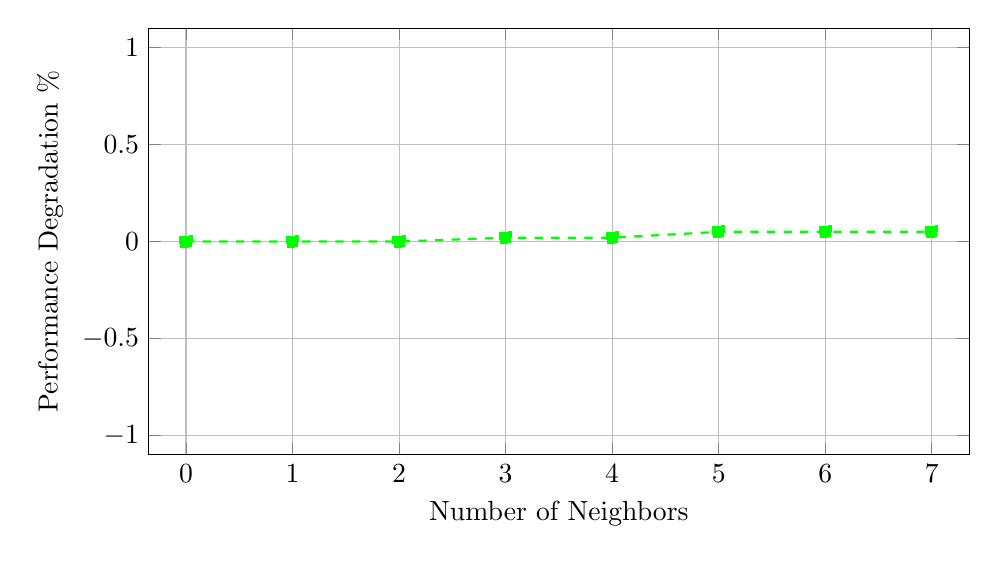
\begin{tikzpicture}
\begin{axis}[
    width=12cm,
    height=7cm,
    xlabel={Number of Neighbors},
    ymin=-1,
    ymax=1, 
    ylabel={Performance Degradation \%},
    grid=both,
    enlargelimits=0.05,
    legend style={at={(0.5,-0.25)}, anchor=north, legend columns=2}
]

\addplot[
    color=green,
    mark=square*,
    dashed,
    thick
] coordinates {
    (0, 0)
    (1, 0)
    (2, 0)
    (3, 0.02)
    (4, 0.02)
    (5, 0.05)
    (6, 0.05)
    (7, 0.05)
};


\end{axis}
\end{tikzpicture}
\caption{Effect of adding busy neighbors on the CPU performance with m6g.2xlarge instances using the cpu\_burn tool}
\end{figure}
\noindent
We notice a very small and insignificant performance  degradation of 0.05\%. This should be due 
to hypervisor overhead which, as claimed by AWS, is practically non-existent. 
The following table captures the final performance degradation for different instances types. 
At each level, we repeated the cpu\_burn command 10 times and then considered the average of these 10 values. 
\begin{table}[H]
\begin{center}
\begin{tabular}{ c|c|c|c|c|c|c }
 Instance type & medium & large & xlarge & 2xlarge & 4xlarge  & 8xlarge  \\
 \hline
 Maximum Nodes & 64 & 32 & 16 & 8 & 4 & 2 \\
\hline
Degradation (Busy) \%& 0.05 & 0.03 & 0 & 0 & 0 & 0  \\
\end{tabular}
\end{center}
\caption{Maximum achievable performance degradation on our test node across various m6g instance types}
\end{table}
\noindent
The results of our experiment prove that the AWS Nitro hypervisor causes practically no overhead and 
the performance is almost indistinguishable from metal as advertised by AWS. We analyze the runtime of 
the different instance type in comparison to running the threads natively on the m6g.metal instance. 
The results can be seen in the following figure. 
\begin{figure}[H]
\centering
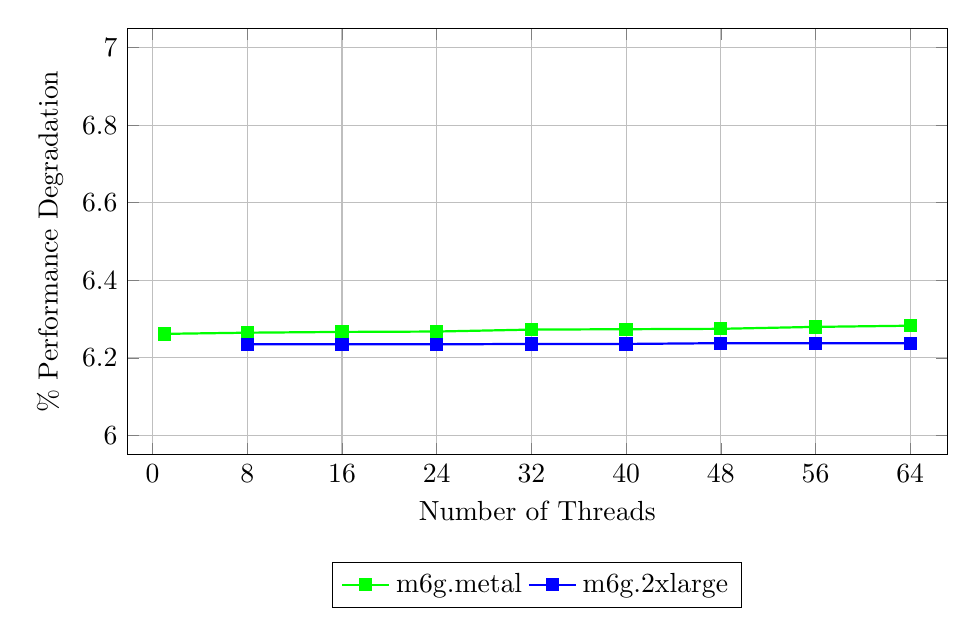
\begin{tikzpicture}
\begin{axis}[
    width=12cm,
    height=7cm,
    xlabel={Number of Threads},
    ylabel={\% Performance Degradation},
    grid=both,
    ymax = 7, 
    ymin = 6,
    xtick distance = 8, 
    enlargelimits=0.05,
    legend style={at={(0.5,-0.25)}, anchor=north, legend columns=2}
]

\addplot[
    color=green,
    mark=square*,
    thick
] coordinates {
    (1, 6.262)
    (8, 6.265)
    (16, 6.267)
    (24, 6.268)
    (32, 6.273)
    (40, 6.274)
    (48, 6.275)
    (56, 6.280)
    (64, 6.283)
};
\addlegendentry{m6g.metal}

\addplot[
    color=blue,
    mark=square*,
    thick
] coordinates {
    (8, 6.235)
    (16, 6.235)
    (24, 6.235)
    (32, 6.236)
    (40, 6.236)
    (48, 6.238)
    (56, 6.238)
    (64, 6.238)
};
\addlegendentry{m6g.2xlarge}


\end{axis}
\end{tikzpicture}
\caption{Effect of adding threads on the CPU performance using m6g.metal and the cpu\_burn tool}
\end{figure}
\noindent
We notice a very little performance degradation on the total execution runtime, reaching a maximum 
of 0.33\% at 64 threads. This result is expected as each new thread is assigned to an independent 
physical core. since the m6g.metal has 64 physical cores, the added threads before 64 should be 
assigned to an idle core and should practically have no effect on the other threads. We even notice 
that the m6g.2xlarge had better performance throughout the experiment. However it's a very 
small difference, which is almost insignificant. 